\chapter{Implementación}
\label{chap:implementacion}

\lettrine{I}{mplementación} es la ejecución o puesta en marcha de una idea programada. Y de ello habla este capítulo: la documentación de la puesta en marcha de lo planeado en el capítulo anterior. Primero se ha de crear el soporte hardware, para posterioremente desplegar el software sobre este mismo.

Como se comenta posteriormente en (TODO \#REF\# metodología), se sigue un modelo basado en prototipos, en el que se realiza un codiseño hardware y software mediante el uso de máquinas virtuales.

\section{Configuración Hardware}
\label{sec:impl_infra_hardware}
\subsection{Preparación}
Como se comenta en \nameref{ssec:diseño_estructural}, el objetivo es construir un cluster compacto, y para ello las diferentes partes se ensamblan por separado. Podemos distinguir así cinco fases:
\begin{itemize}
    \item Montaje de las torres de Raspberry Pi: Se debe montar cada piso de la torre, acomodando cada Raspberry en cada nivel (es decir, colocando disipadores, anclajes, y conectores magnéticos USB) como se muestra en la figura \ref{fig:modulo_raspi_torre}, donde se ve un módulo de la torre. Asimismo, en la figura \ref{fig:proceso_apilamiento} se puede ver el proceso de apilamiento.

    \begin{figure}[h!]
    \centering
    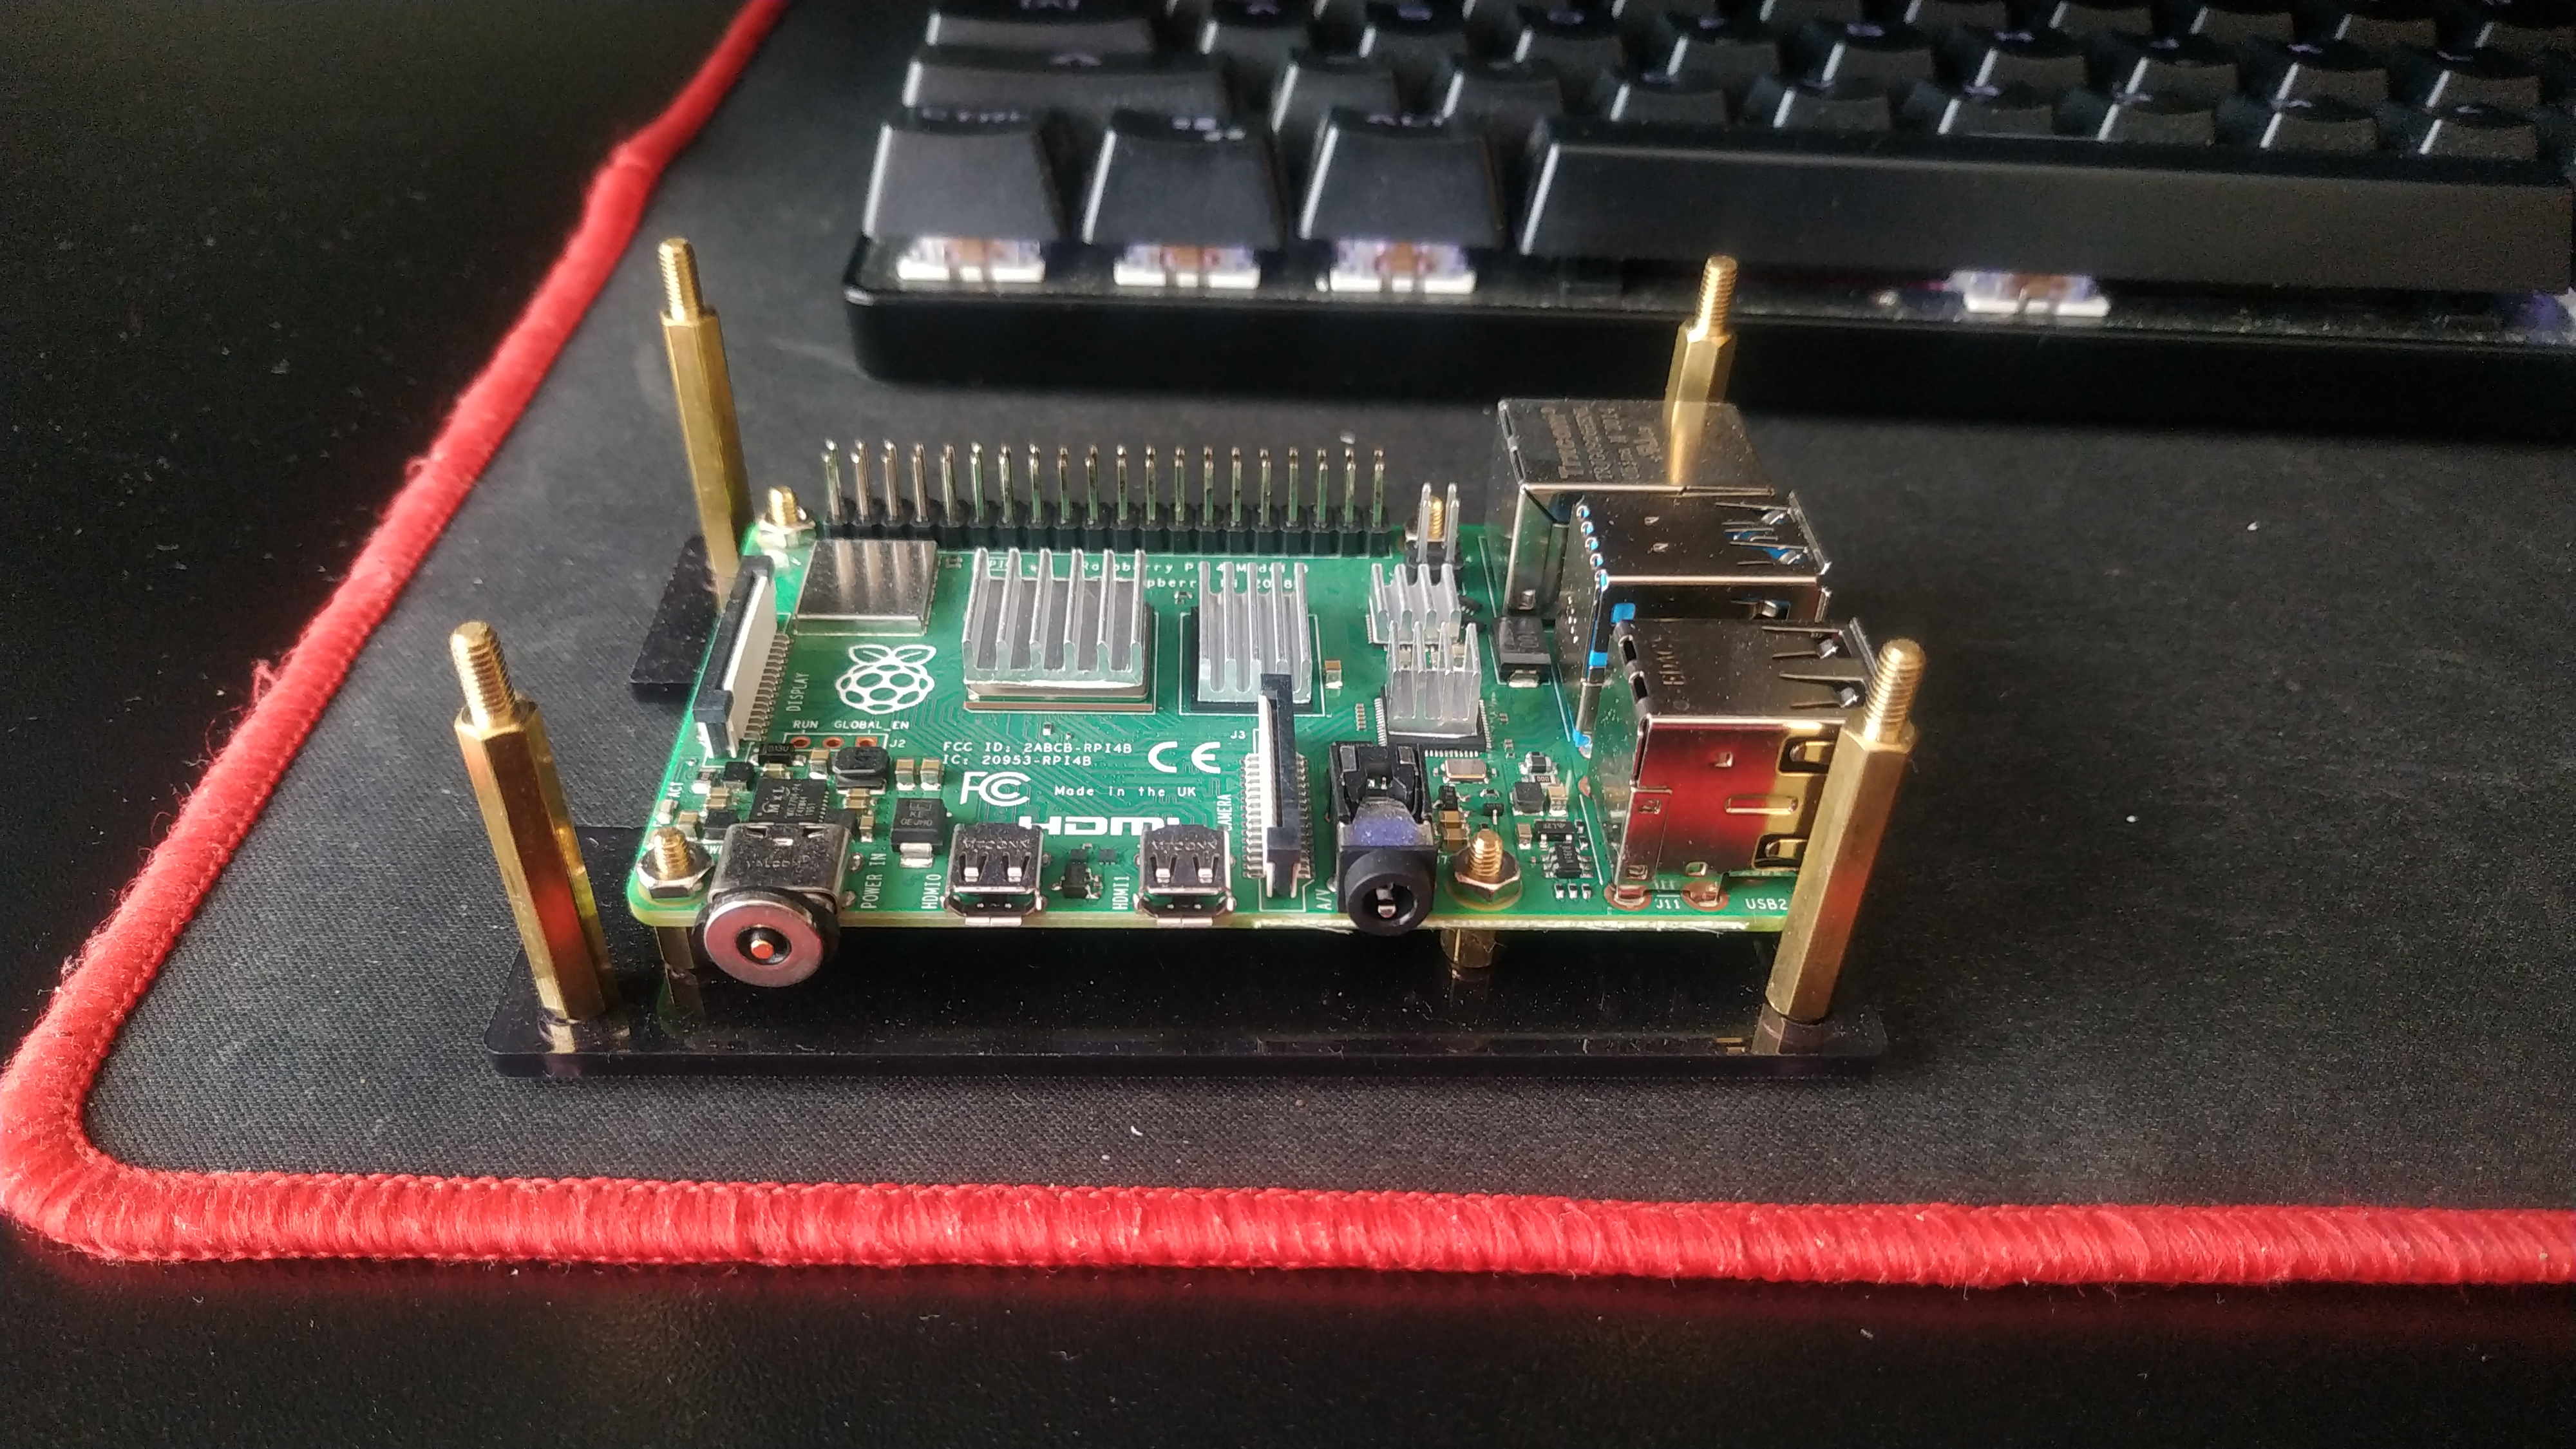
\includegraphics[width=0.8\textwidth]{img/modulo_raspi_torre.jpg}
    \caption{Un módulo de la torre completamente ensamblado}
    \label{fig:modulo_raspi_torre}
    \end{figure}

    \begin{figure}[h!]
    \centering
    \begin{subfigure}[c]{0.4\textwidth}
        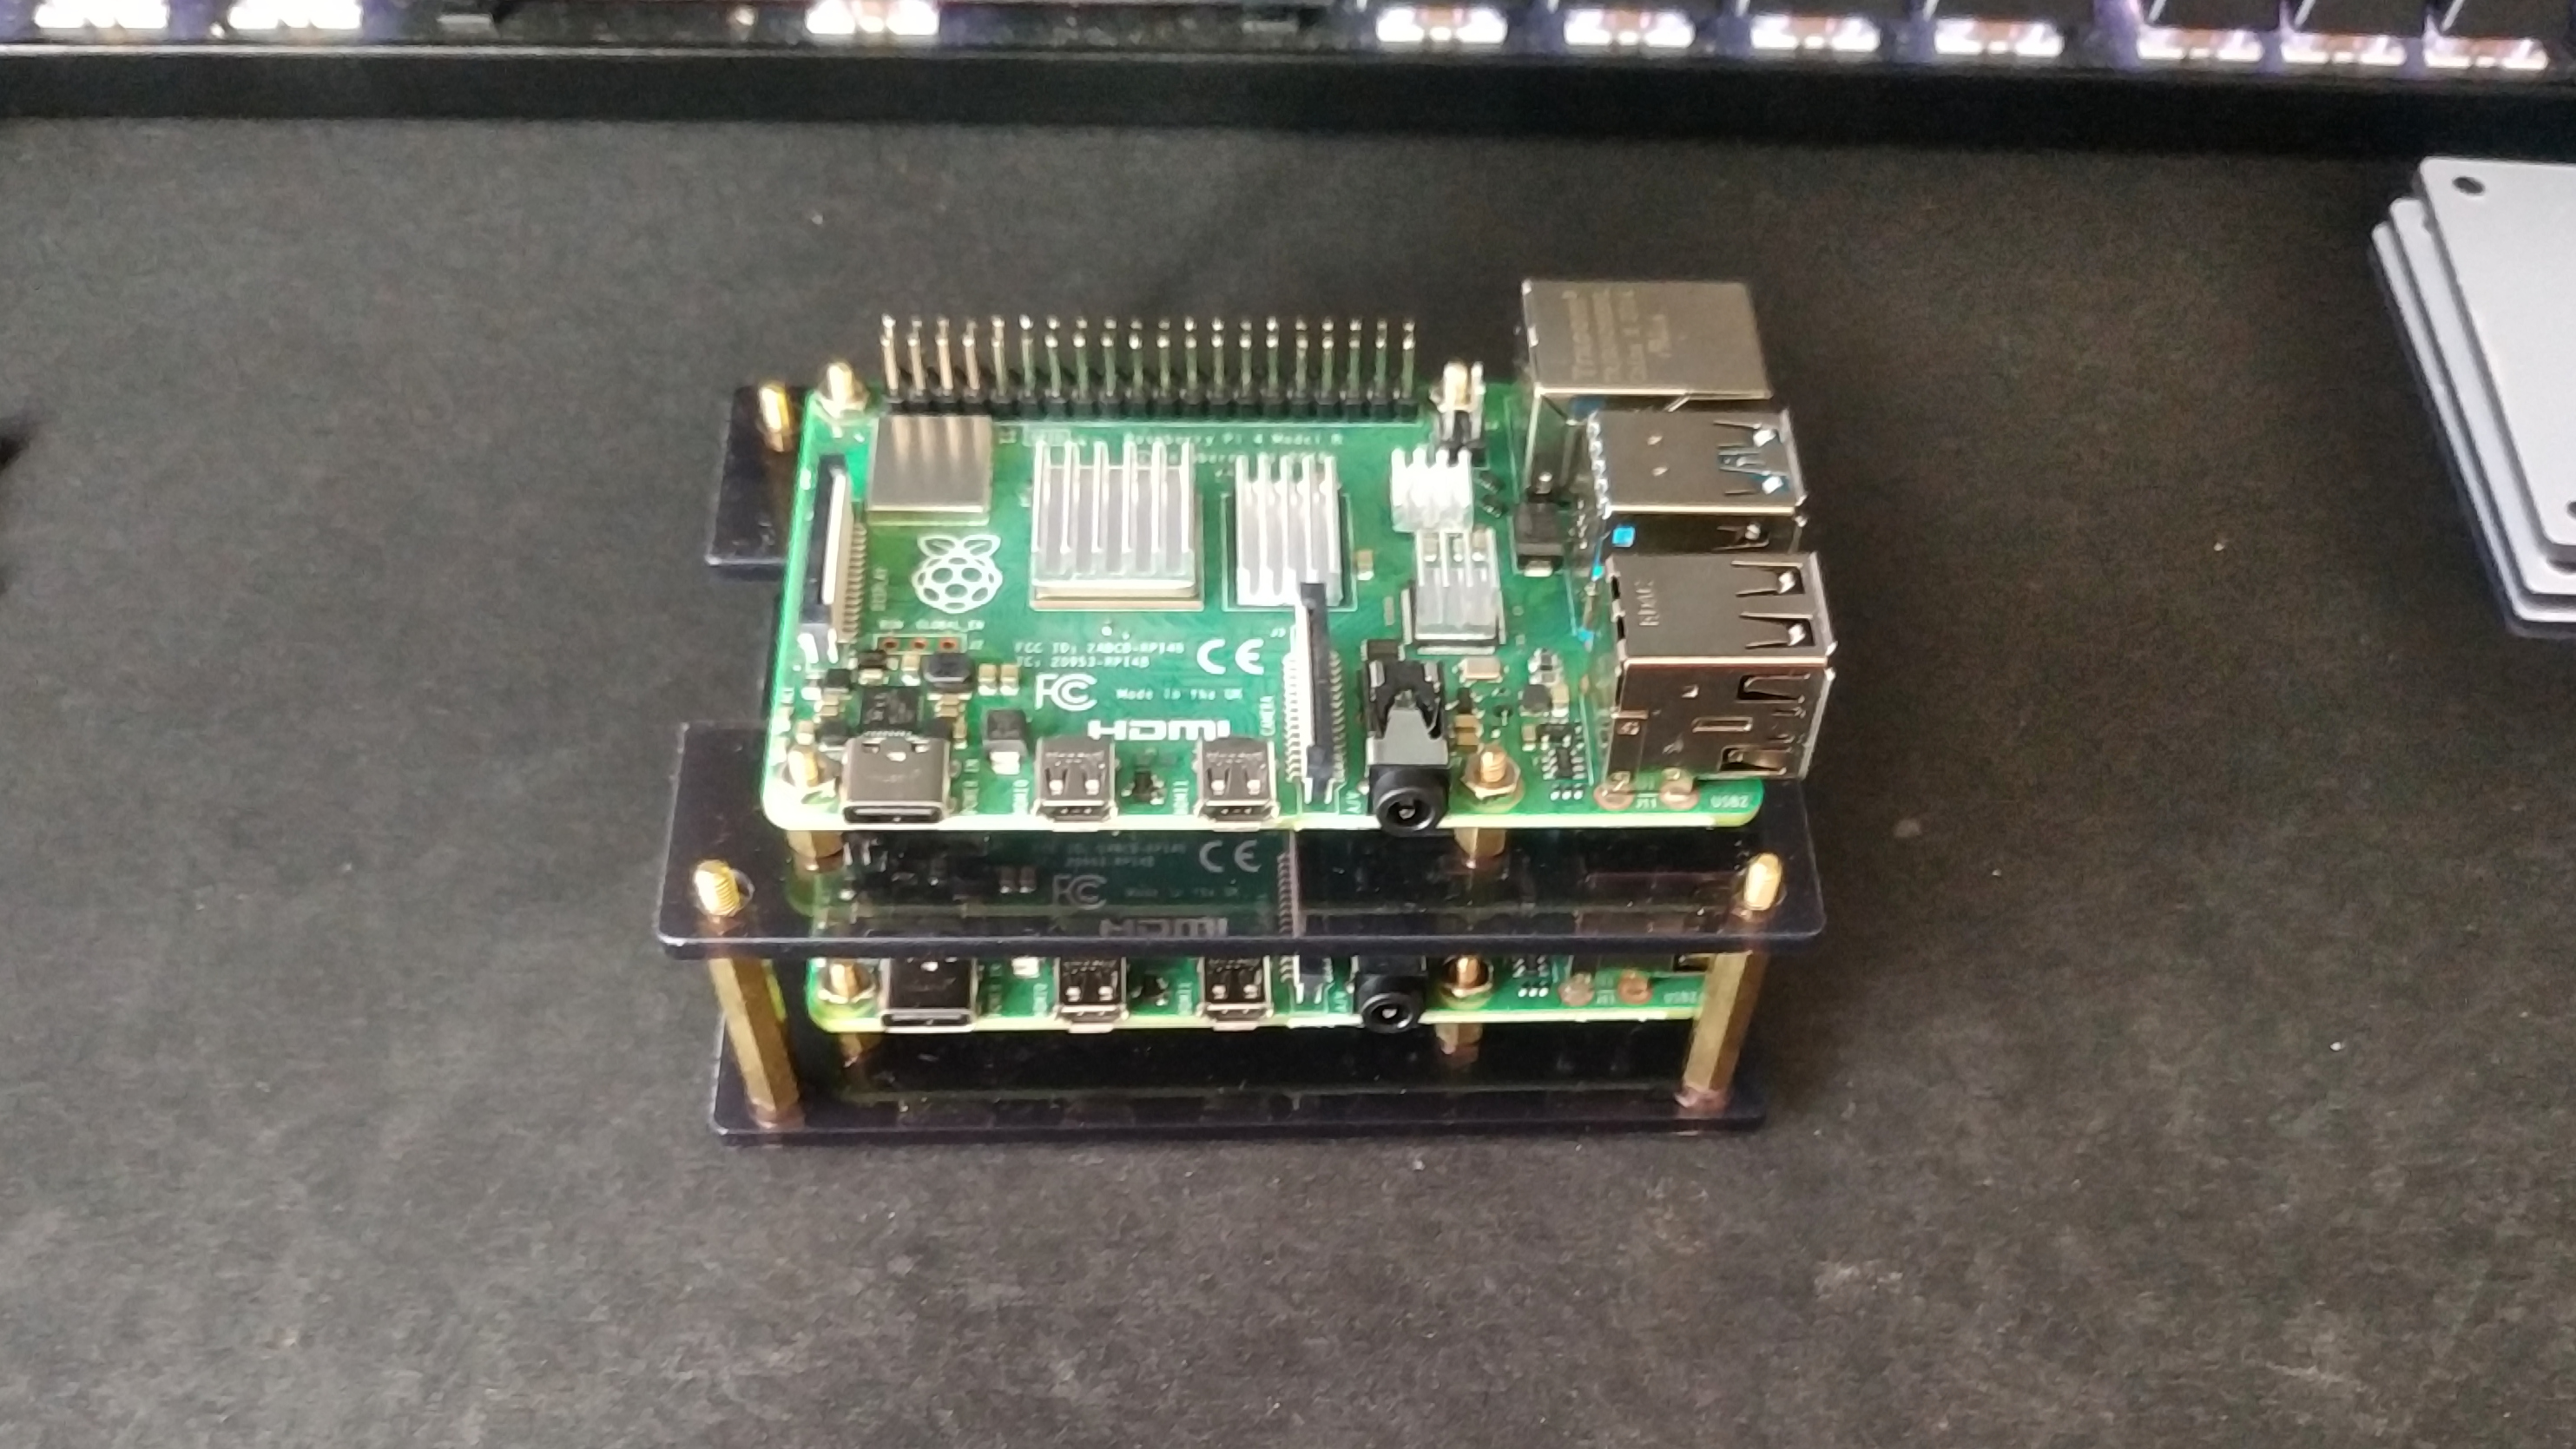
\includegraphics[width=\textwidth]{img/apilamiento/2.jpg}
        \caption{Dos Raspberry Pis apiladas}
        \label{fig:apilamiento_2}
    \end{subfigure}
    \begin{subfigure}[c]{0.4\textwidth}
        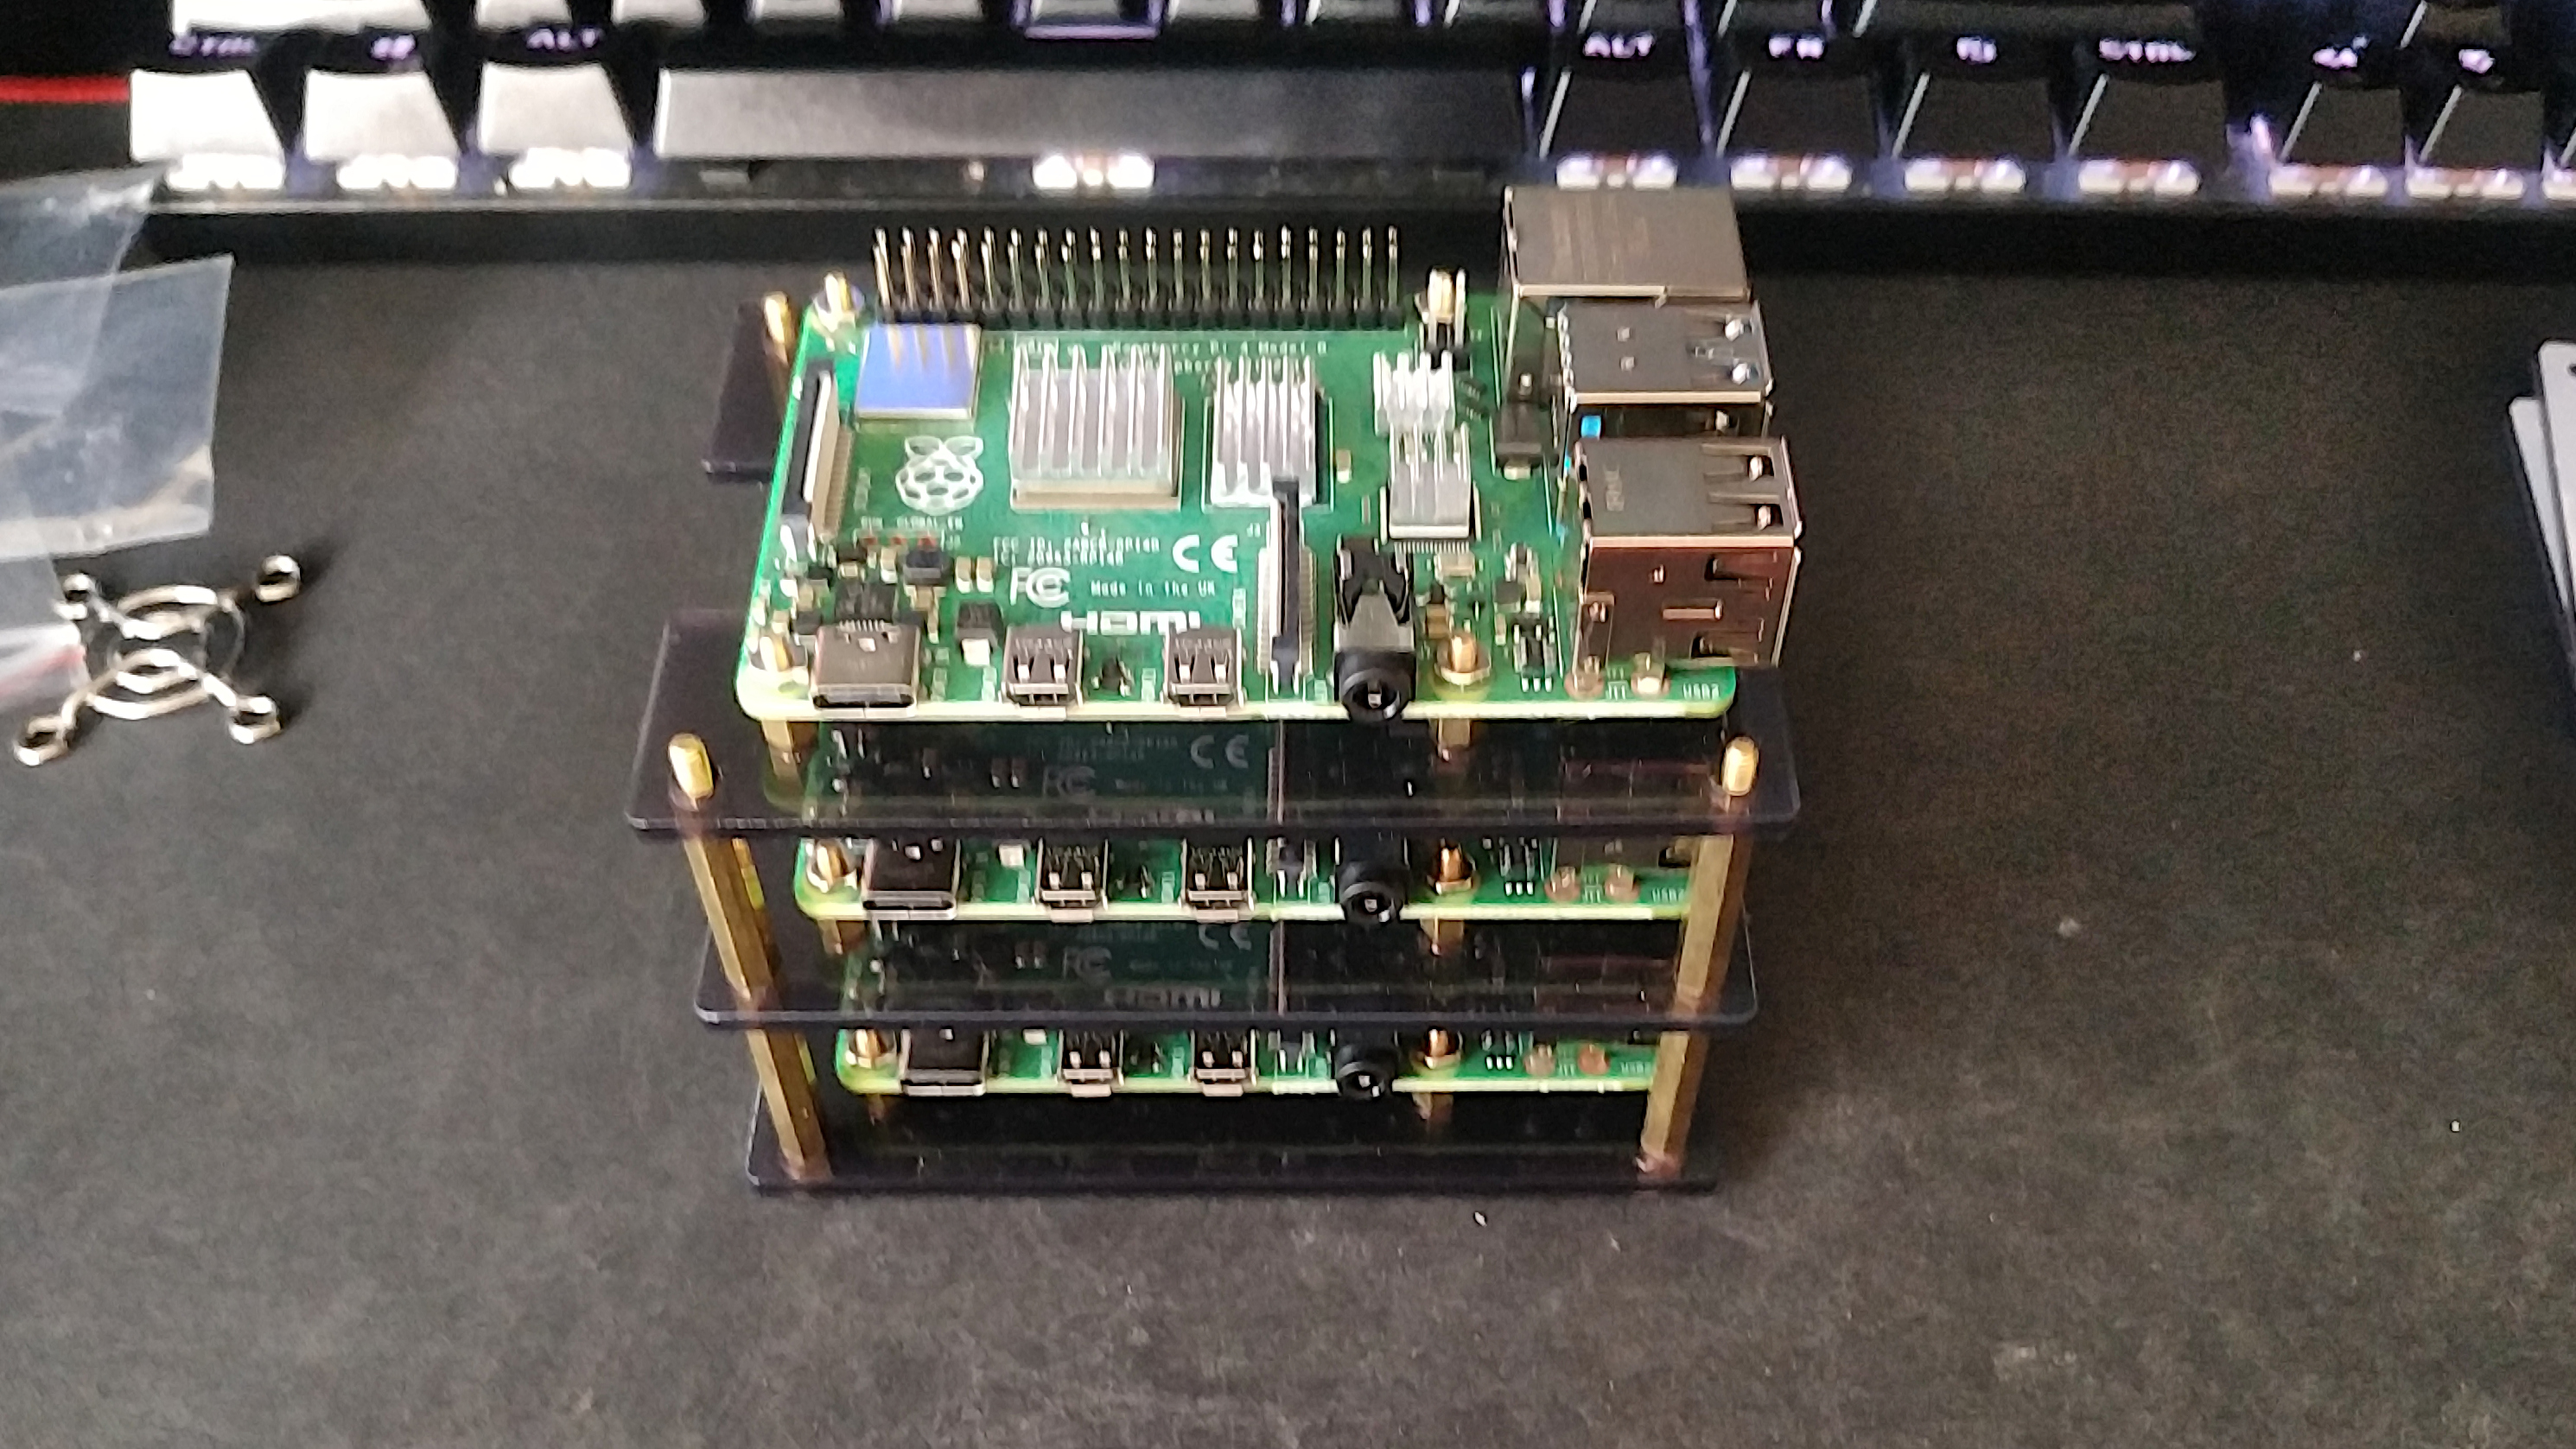
\includegraphics[width=\textwidth]{img/apilamiento/3.jpg}
        \caption{Tres}
        \label{fig:apilamiento_3}
    \end{subfigure}

    \begin{subfigure}[c]{0.4\textwidth}
        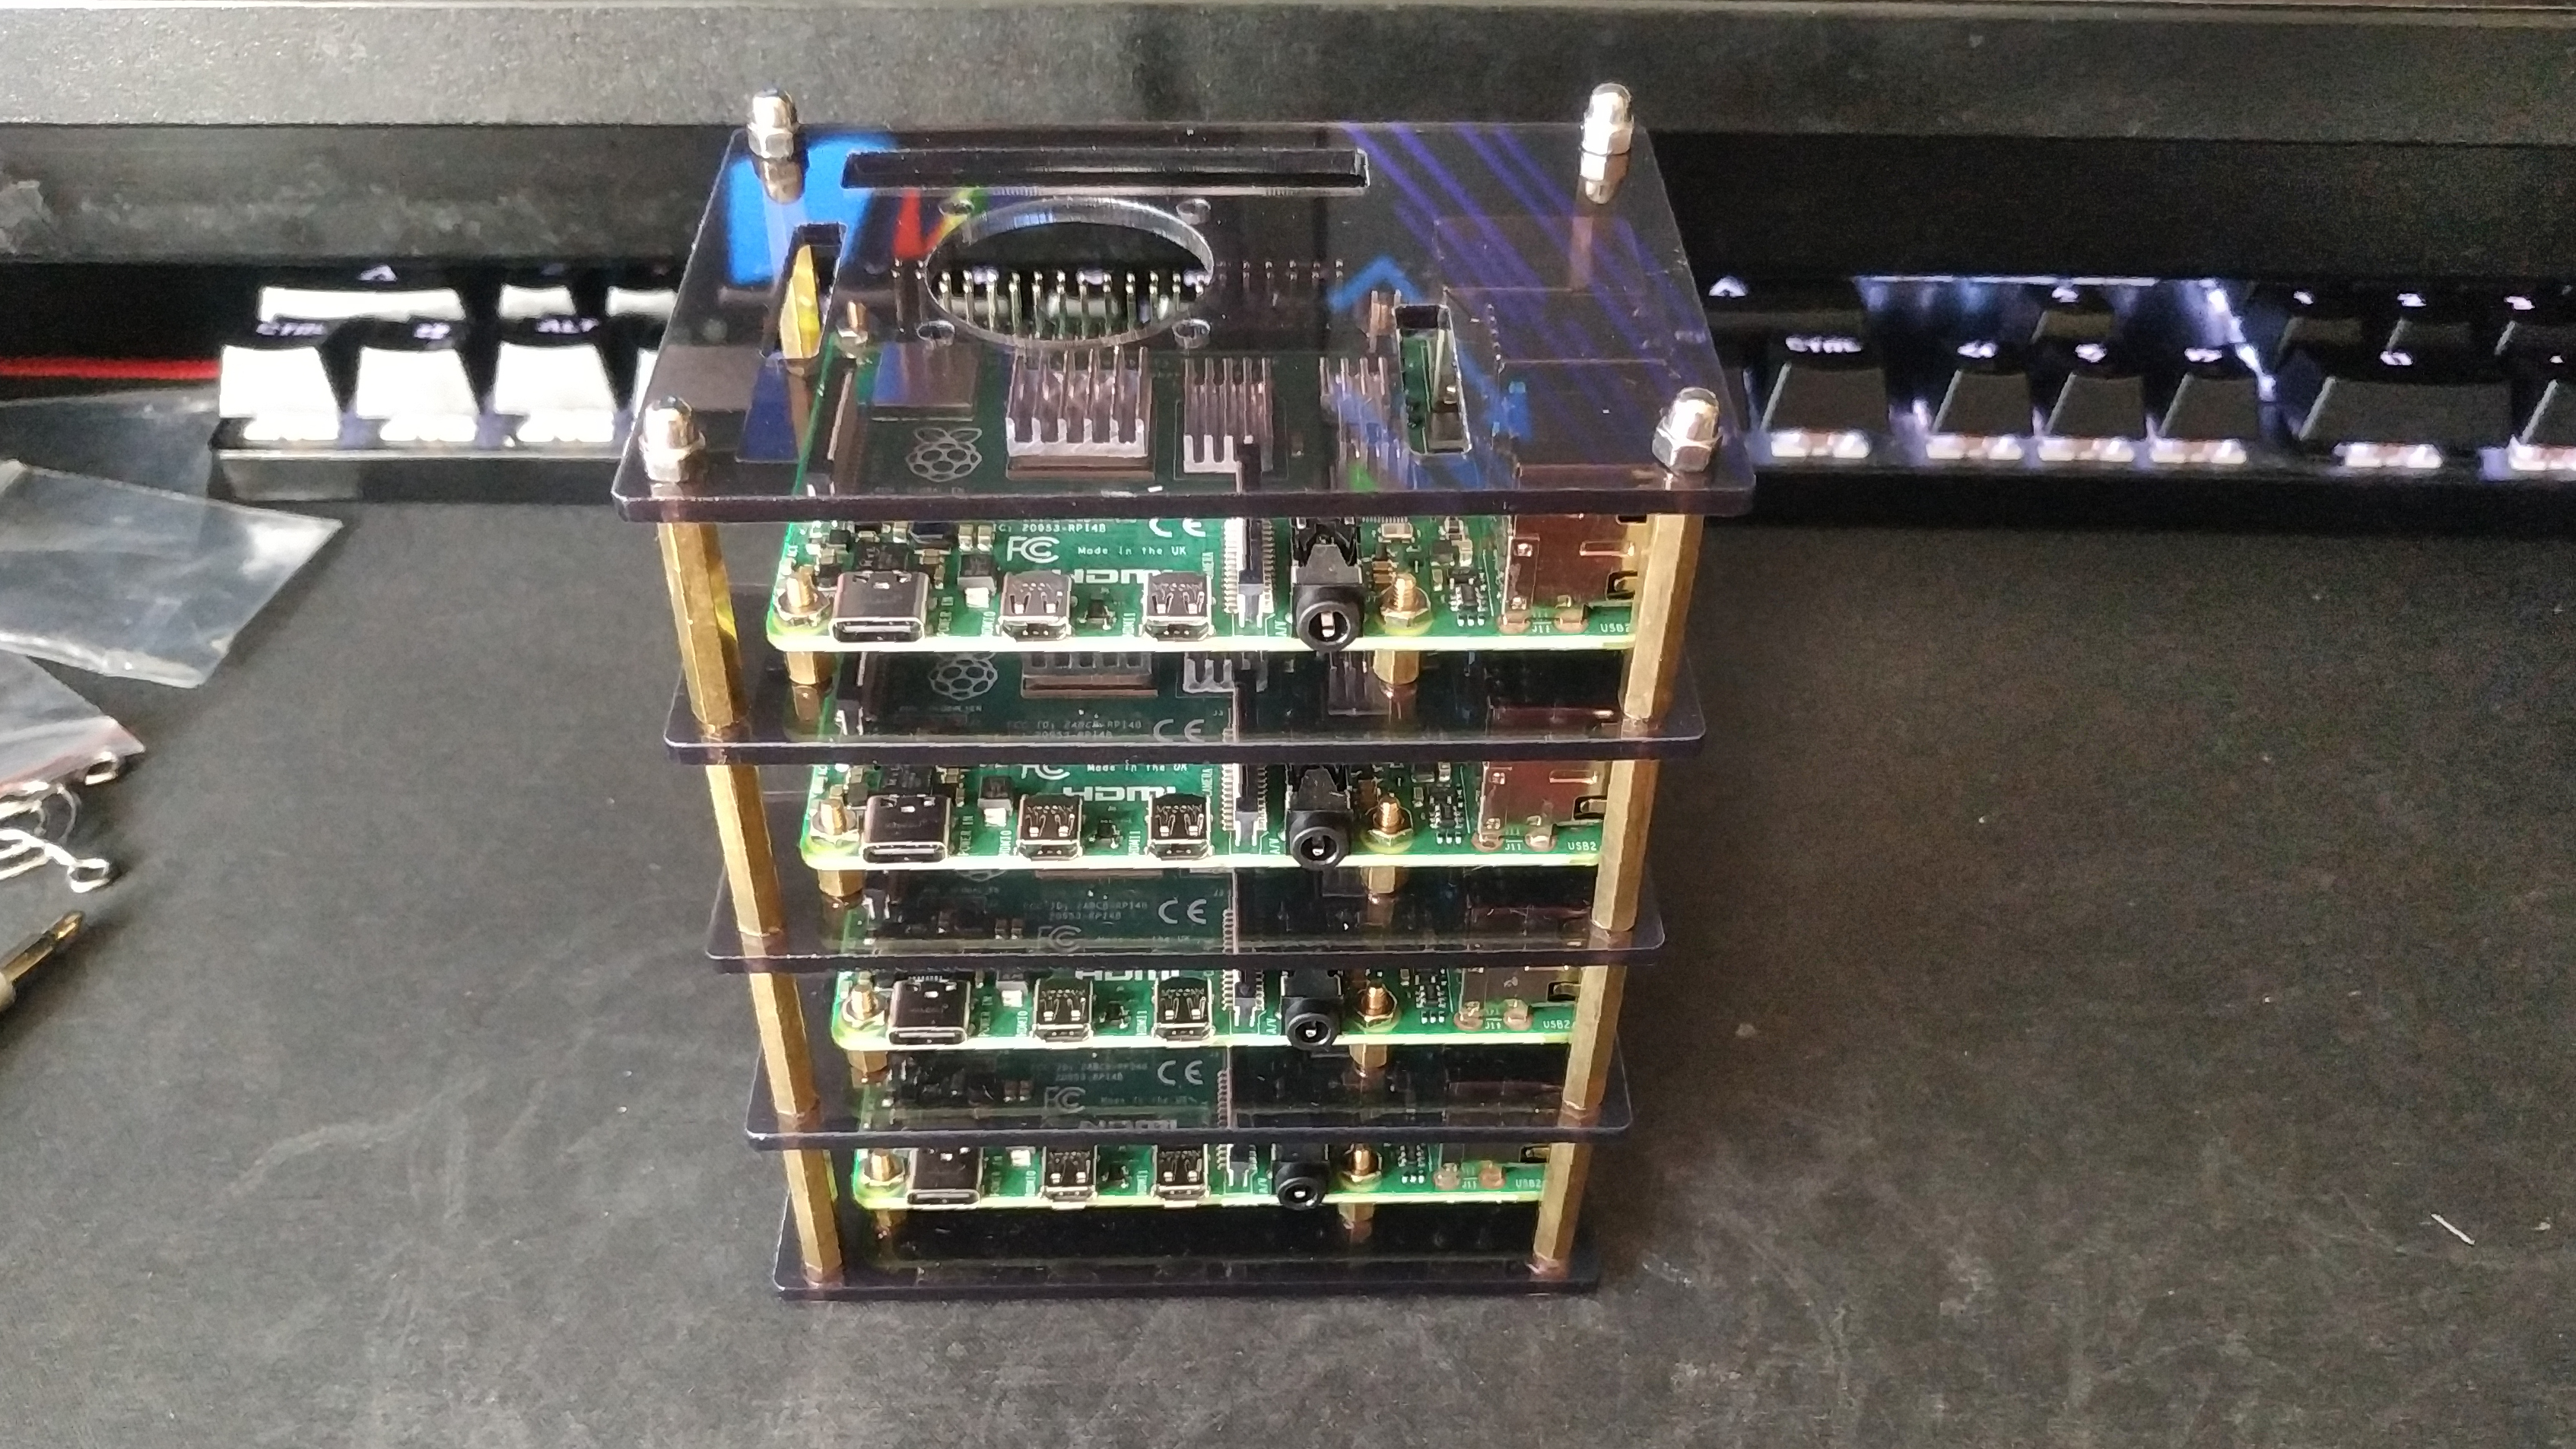
\includegraphics[width=\textwidth]{img/apilamiento/4.jpg}
        \caption{Primera torre completa}
        \label{fig:apilamiento_4}
    \end{subfigure}
    \begin{subfigure}[c]{0.4\textwidth}
        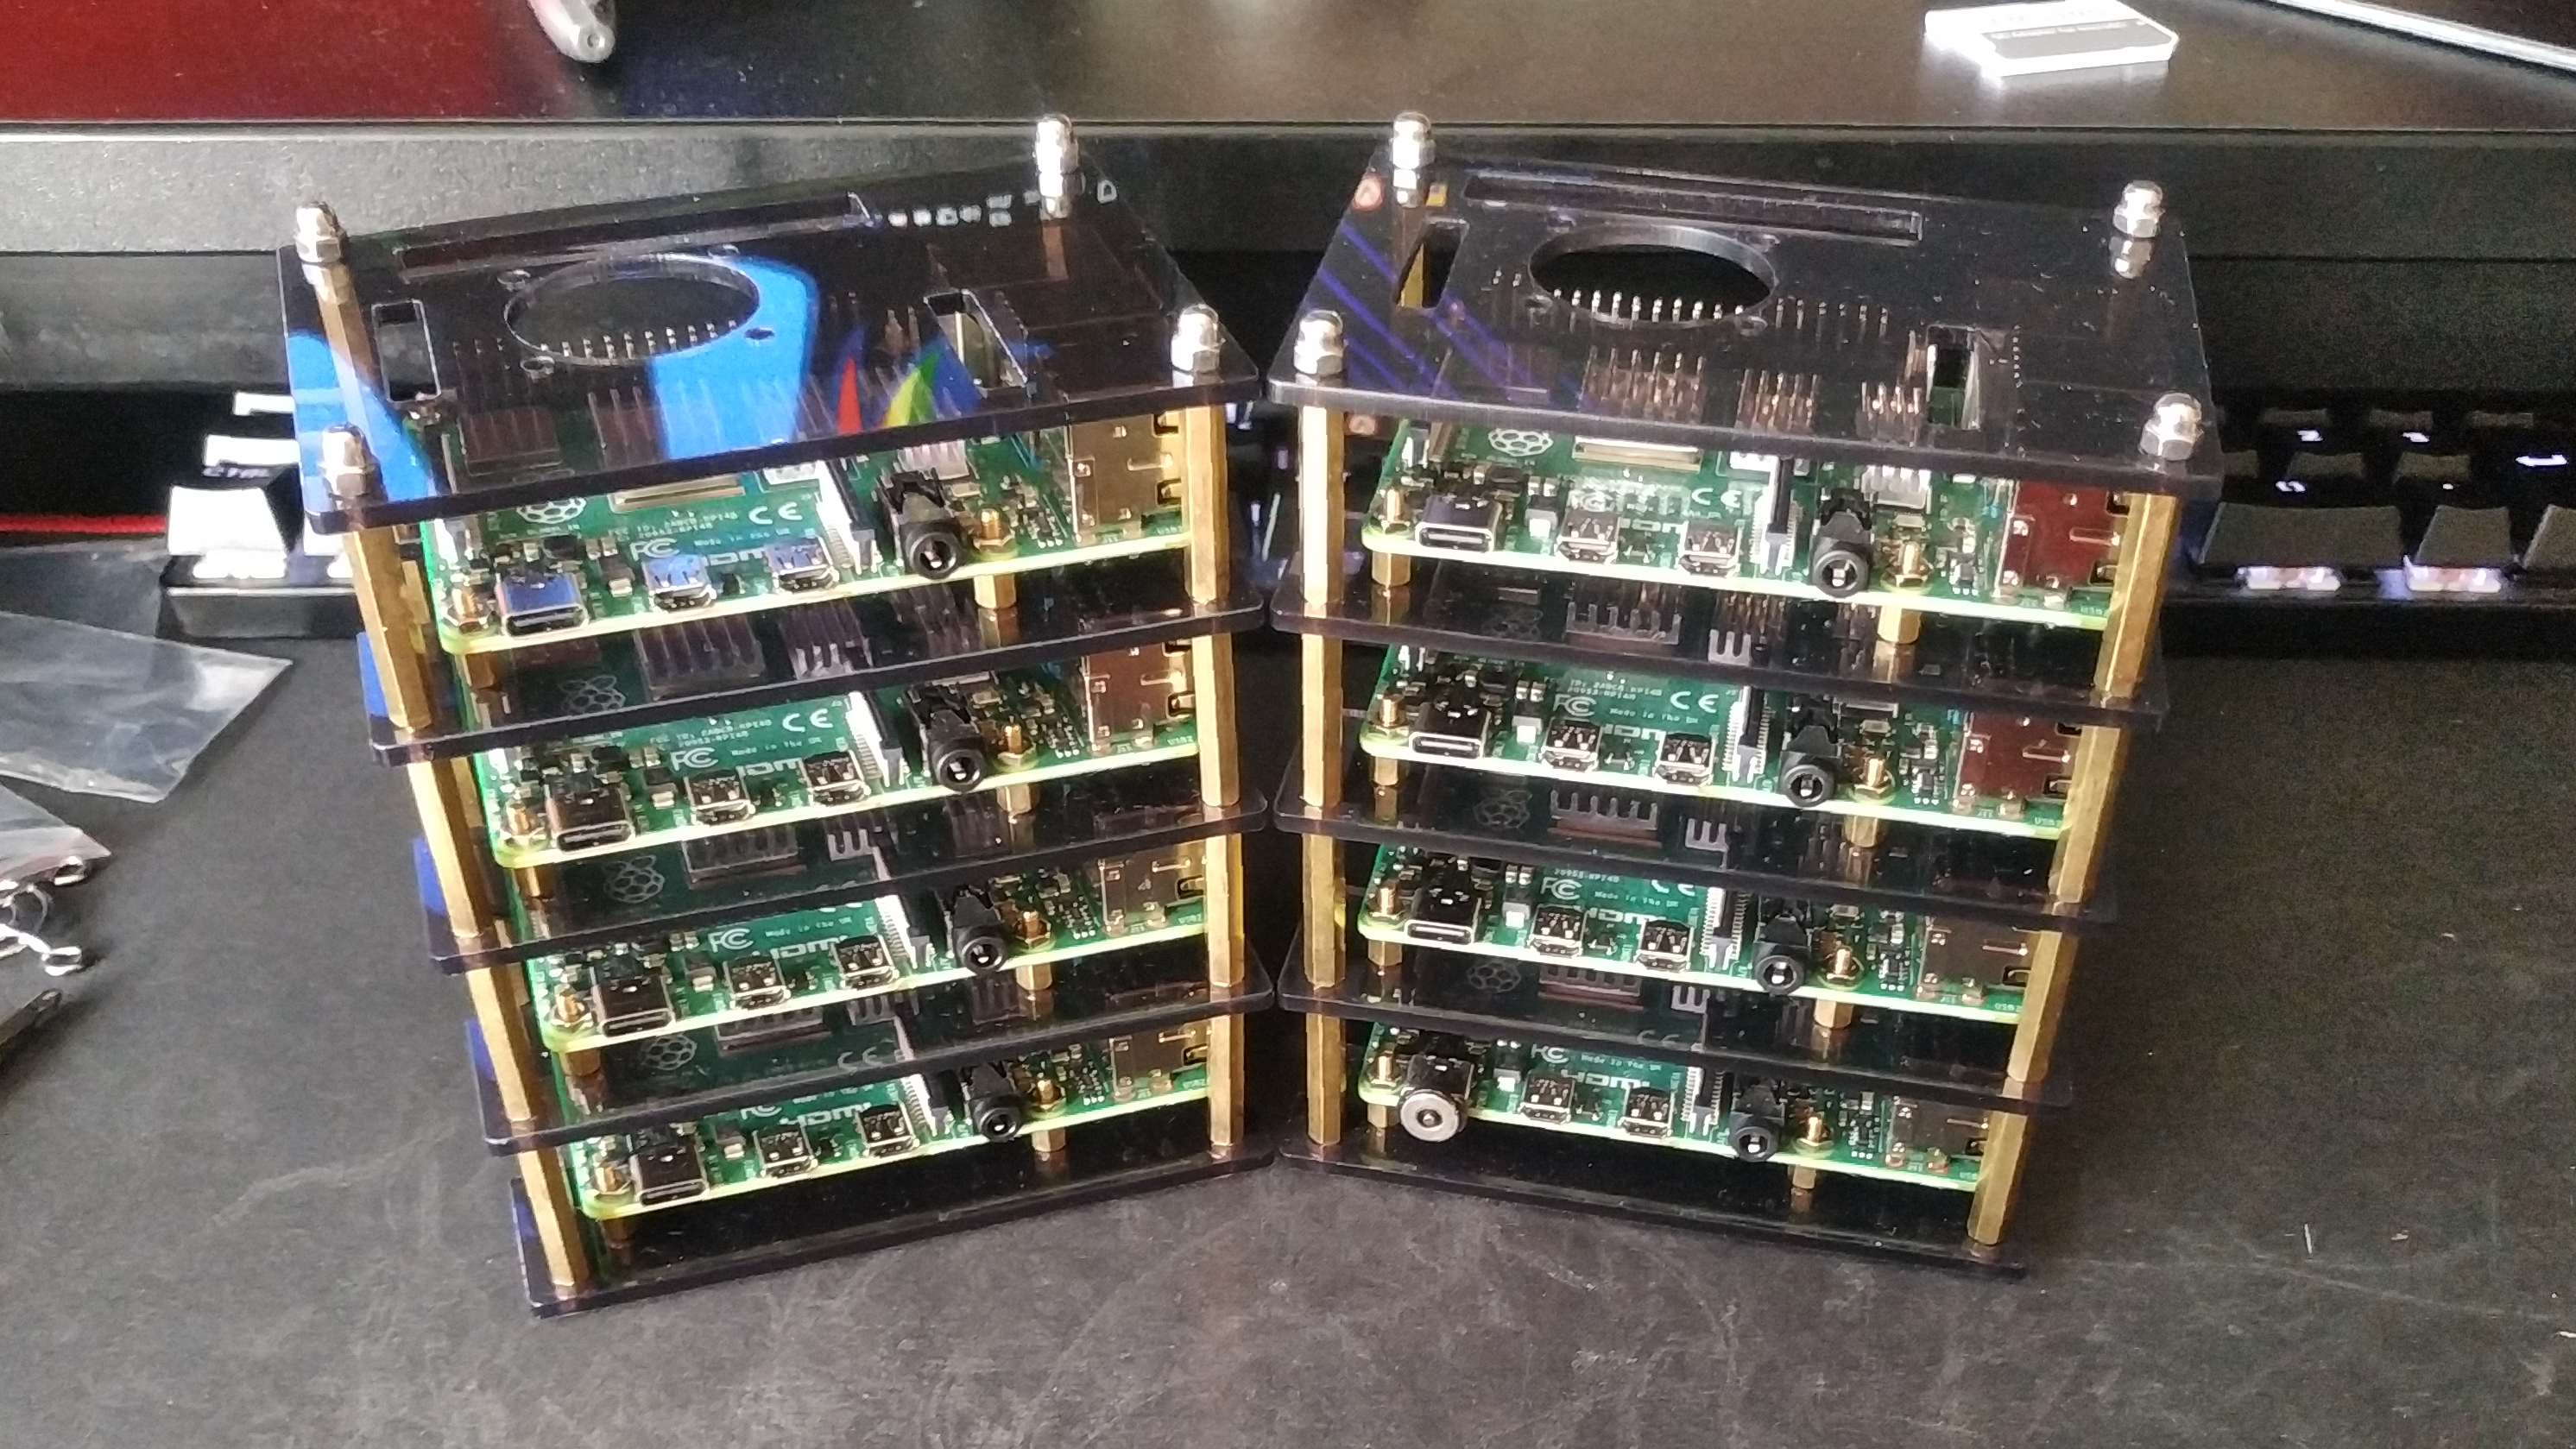
\includegraphics[width=\textwidth]{img/apilamiento/8.jpg}
        \caption{Y ambas torres}
        \label{fig:apilamiento_8}
    \end{subfigure}
    \caption{Proceso de apilamiento de las torres de Raspberry Pis}
    \label{fig:proceso_apilamiento}
    \end{figure}
    
    \item Testeo del correcto funcionamiento
    \item Cortado de las láminas adaptadoras de aluminio
    \item Ensamblado final y cableado
    \item Testeo de correcta integración
\end{itemize}

\section{Configuración Software}
\label{sec:impl_infra_software}

\subsection{Instalación Base del Sistema Operativo}
\label{ssec:instalacion_sistema_operativo}
Para instalar Arch Linux en las Raspberry Pi 4, deberemos ir a la página web de ArchLinuxARM\footnote{\url{https://archlinuxarm.org/platforms/armv8/broadcom/raspberry-pi-4}} y seguir las instrucciones. En nuestro caso, al no tener dependencias fuertes en las librerías de 32 bits, optamos por la versión de 64 bits, que nos otorgará mayor rendimiento.

Así, asumiendo que conectamos en \texttt{/dev/sdd} la tarjeta microSD donde flashearemos Arch Linux, primeramente descargaremos el sistema de archivos de Arch

\begin{lstlisting}[language=bash,basicstyle=\scriptsize]
wget http://os.archlinuxarm.org/os/ArchLinuxARM-rpi-aarch64-latest.tar.gz
\end{lstlisting}

y tras ello ejecutamos para cada una de las tarjetas:

\begin{lstlisting}[language=bash]
#!/bin/sh

MICROSD=/dev/sdd

echo "Ejecutando sobre ${MICROSD}"

sed -e 's/\s*\([\+0-9a-zA-Z]*\).*/\1/' << EOF | fdisk ${MICROSD}
    o       # Limpiamos la tabla de particiones
    n       # Creamos una nueva partición
    p       #  primaria
    1       #  número uno
            #  por defecto al principio del disco
    +200M   #  y con un tamaño de 200MiB
    t       # Cambiamos el tipo de la partición
    c       #  a W95 FAT32 (LBA)
    n       # Creamos otra partición
    p       #  primaria
    2       #  número dos
            #  a continuación de la primera
            #  y que ocupe todo el disco
    w       # Escribmos la tabla de particiones
EOF

# Creamos carpetas para montar las particiones 1 (boot) y 2 (boot)
mkdir -p boot root

# Y creamos los sistemas de ficheros
mkfs.vfat ${MICROSD}1
mkfs.ext4 ${MICROSD}2

# Montamos las particiones
mount ${MICROSD}1 boot
mount ${MICROSD}2 root

# Y extraemos el tarball a root
bsdtar -xpf ArchLinuxARM-rpi-aarch64-latest.tar.gz -C root

# Movemos el directorio boot a su partición
mv root/boot/* boot

# Hacemos una modificación en el fstab para adaptarlo a los 64 bits
sed -i 's/mmcblk0/mmcblk1/g' root/etc/fstab

# Escribimos los datos a la SD y desmontamos las carpetas
sync
umount boot root
\end{lstlisting}

Tras ello conectamos el cluster (desconectando una Raspberry del switch y conectando un cable) a nuestra red ya existente y los encontramos con:

\begin{lstlisting}[language=bash]
nmap  -sP -PR 192.168.0.*    
\end{lstlisting}

De esta forma podremos hacer ssh a cada uno de ellos y prepararlos para el uso, actualizandolos y preparándolos para el uso:\footnote{Contraseñas \texttt{alarm:alarm}, \texttt{root:root}}

\begin{lstlisting}[language=bash]
ssh alarm@<IP>
su -                # Nos hacemos root

# Inicializamos y poblamos el keyring para el gestor de paquetes
pacman-key --init
pacman-key --populate archlinuxarm

# Y actualizamos el sistema a la última versión
pacman -Syyu

# Aprovechamos para cambiar el hostname del sistema
#  Seguiremos el esquema de nombres rpiX, siendo la 0 y 1
#   - rpi0
#   - rpi1
echo rpiX > /etc/hostname

# Esto como algo más personal, pero que mejora ligeramente la experiencia en las actualizaciones, editamos el archivo /etc/pacman.conf
#  Y descomentamos
#   Color
#   ParallelDownloads (y lo dejamos al valor predeterminado de 5)
nano /etc/pacman.conf

# Tras esto el sistema debe reiniciarse para cargar el (más que probable) kernel actualizado
reboot
\end{lstlisting}

\subsection{Bridging de Interfaces}
Como el switch tiene el mismo número de puertos que el número de Raspberries, se necesita una forma de conectar el cluster a un ordenador externo. Para esto se puentea el adaptador USB 3.0 a Gigabit Ethernet que se puede conectar en cualquier puerto del nodo maestro (rpi0).

Las configuraciones a realizar en \texttt{/etc/systemd/network} son las siguientes:

\begin{itemize}
    \item Desactivar DHCP en las reglas para ethernet \texttt{en.network} y \texttt{eth.network}, y activarles el bridge maestro en \texttt{br0}:
\begin{lstlisting}[language=bash]
...

[Network]
Bridge=br0
#DHCP=yes
#DNSSEC=no
\end{lstlisting}
    \item Crear el network device \texttt{br0.netdev}
\begin{lstlisting}[language=bash]
[NetDev]
Name=br0
Kind=bridge
\end{lstlisting}
    \item Y asignar una IP al bridge en \texttt{br0.network}
\begin{lstlisting}[language=bash]
[Match]
Name=br0

[Network]
DHCP=yes
DNSSEC=no
\end{lstlisting}
\end{itemize}

Tras realizar estas configuraciones se reinicia \texttt{systemd-networkd} con
\begin{lstlisting}[language=bash]
systemctl restart systemd-networkd
\end{lstlisting}

Y (probablemente) se deba reconectar la sesión por SSH, ya que al haber cambiado la MAC de la interfaz, el servidor DHCP en uso le habrá cambiado también la IP asignada a rpi0.

\subsection{Configuración de direcciones IP estáticas}
\label{ssec:configuracion_ip_estaticas}
A la hora de administrar el cluster es necesario que las direcciones se asignen de alguna forma, sea esta estática o dinámica. Sin embargo, debido a las características del cluster, y especialmente a que la conexión desde el exterior va a ser variable y no siempre va a haber internet, lo más conveniente es configurar direcciones IP estáticas en cada uno de los hosts que componen el cluster, así como una dirección de gateway predeterminada, que algunas veces existirá, y otras no.

Para esto, se han de modificar los archvos ubicados en \texttt{/etc/systemd/network/} de tal forma que:

\begin{itemize}
    \item Modificar \texttt{eth.network} en las máquinas 1 a 7, y asignarles una IP estática, siendo la X en \texttt{.22X} el número de la máquina, así \texttt{rpi1} sería \texttt{.221}, etc.
\begin{lstlisting}[language=bash]
[Match]
Name=eth*

[Network]
Address=192.168.0.22X/24
Gateway=192.168.0.1
DNS=8.8.8.8
#DHCP=yes
#DNSSEC=no
\end{lstlisting}
    \item Proceder de igual forma con el bridge en el nodo maestro, asignando una IP estática al bridge en \texttt{br0.network}:
\begin{lstlisting}[language=bash]
[Match]
Name=br0

[Network]
Address=192.168.0.220/24
Gateway=192.168.0.1
DNS=8.8.8.8
#DHCP=yes
#DNSSEC=no
\end{lstlisting}
\end{itemize}

\subsection{Escritura del fichero /etc/hosts}
Para hacer referencia al resto de raspberries sin necesidad de escribir su dirección IP (lo que será útil más adelante para la ejecución de tareas con MPI), es conveniente agregar una entrada por raspberry pi a cada una de ellas en el fichero \texttt{/etc/hosts} para poder referenciarlas por su nombre.

De esta manera, ejecutamos
\begin{lstlisting}[language=bash]
cat << EOS >> /etc/hosts
127.0.0.1       localhost
192.168.0.220   rpi0
192.168.0.221   rpi1
192.168.0.222   rpi2
192.168.0.223   rpi3
192.168.0.224   rpi4
192.168.0.225   rpi5
192.168.0.226   rpi6
192.168.0.227   rpi7
EOS
\end{lstlisting}

\subsection{Creación del usuario mpiuser}
Actualmente contamos con dos usuarios, \texttt{root} y \texttt{alarm}, ninguno de los cuales es apto para lanzar las tareas mpi: El primero no es recomendable su uso para tareas que no lo requieran así, y el segundo es el que se utiliza como usuario por defecto no privilegiado, por lo que es conveniente crear un tercero que se encargue del lanzamiento de las tareas mpi: \texttt{mpiuser}.

Para ello ejecutamos en todos los nodos
\begin{lstlisting}[language=bash]
# Creamos el usuario mpiuser y su carpeta en /home
useradd -m mpiuser
# Y le asignamos la contraseña mpi
echo "mpiuser:mpi" | chpasswd
\end{lstlisting}

\subsection{Generación de claves SSH}
Tras la creación de los usuarios para la ejecución de tareas paralelas con mpi, debemos configurar la autenticación no interactiva mediante SSH. Esto se realiza con autenticación mediante par de claves pública y privada.

Sabiendo esto, deberemos ejecutar en todos los nodos del cluster como usuario \texttt{mpiuser} (\texttt{su - mpiuser})
\begin{lstlisting}[language=bash]
ssh-keygen
\end{lstlisting}

Como será el nodo maestro el que lance las tareas, debemos copiar la clave pública del nodo maestro al resto de nodos, lo cual se puede semi-automatizar con el siguiente comando:

\begin{lstlisting}[language=bash]
for i in {1..7}; do
    ssh-copy-id mpiuser@rpi$i
done
\end{lstlisting}

Y comprobaremos que se han copiado satisfactoriamente a todos los nodos con
\begin{lstlisting}[language=bash]
for i in {1..7}; do
    ssh mpiuser@rpi$i "cat /etc/hostname"
done
\end{lstlisting}
Este último comando debería mostrar los hostnames del resto de nodos del cluster, sin interrumpir al usuario preguntando contraseña, es decir, en modo no-interactivo.


\subsection{Servidor NFS}
Debido a que las llamadas a \texttt{mpirun} con múltiples hosts ejecutan el mismo comando en todos ellos, debemos tener algún tipo de almacenamiento compartido, y bajo el mismo nombre, para que al ejecutar el mismo comando, abran el mismo ejecutable. Por tanto el último paso a realizar para poder comenzar con la ejecución de benchmarks es montar algún tipo de almacenamiento compartido, siendo la elección NFS.

El servidor será el nodo maestro, y el resto serán clientes. Los pasos a realizar en todos los nodos (como root) son los siguientes:

\begin{lstlisting}[language=bash]
# Instalamos el paquete de NFS en todos los nodos
pacman -S nfs-utils

# Creamos la carpeta /mpishared
mkdir -p /mpishared
chown mpiuser:mpiuser /mpishared
\end{lstlisting}

A continuación ejecutaremos los siguientes comandos en el nodo maestro:

\begin{lstlisting}[language=bash]
# Añadimos la carpeta compartida a exports
echo "/mpishared      192.168.0.0/24(ro,sync,fsid=0)" >> /etc/exports

# Y recargamos los exports
exportfs -arv

# Tras ello activamos e iniciamos el servidor nfs
systemctl enable --now nfs-server.service
\end{lstlisting}

Y añadiremos al fstab del resto de nodos la siguiente línea
\begin{lstlisting}[language=bash]
echo "rpi0:/ /mpishared nfs defaults,timeo=900,retrans=5,x-systemd.requires=network-online.target,_netdev 0 0" >> /etc/fstab
\end{lstlisting}

\subsubsection{Solución de problemas}
Podría parecer que todo está correcto, pero hay un sutil problema en esta configuración: Dependiendo si rpi0 se apaga primero o no, el resto de nodos pueden quedarse esperando a que responda el share de NFS. Solucionar esto es más sencillo de lo que podría parecer: hemos de establecer un pequeño timeout antes de detener el servidor NFS de, por ejemplo, 5 segundos.

\begin{lstlisting}[language=bash]
# Extendemos la unit del servidor nfs
systemctl edit nfs-server.service

# Añadimos en la zona editable
[Service]
ExecStop=
ExecStop=/bin/sleep 5
ExecStop=/usr/sbin/rpc.nfsd 0

# Salimos y ejecutamos
systemctl daemon-reload
\end{lstlisting}